\chapter{Port-Hamiltonian plate (and shell?) theory}

\epigraph{You get tragedy where the tree, instead of bending, breaks.}{\textit{Culture and Value\\
Ludwig Wittgenstein}}
\minitoc

\lettrine{\color{theme}{P}}lates are plane structural element with a small thickness compared to the planar dimension. Because of the thickness smallness, it is not necessary to model plate structure using three-dimensional models. Therefore, dimensional reduction strategies are employed to model plate structures as two-dimensional problems. These strategies rely on a educated guess of the displacement field. Enough freedom is left so that the assumed field satisfies the equations of elasticity. For beams ans plates the displacement field is expressed in terms of unknown functions $\phi_i^j(x,y,t)$ that solely depends on the midplane coordinates $(x,y)$

\[
u_i(x,y,z,y) = \sum_{j=0}^m (z)^j \phi_i^j(x,y,t).
\]
where $u_{i}$ are the component of the displacement field. The unknown functions are determined so to respect the principle of virtual displacement. In this chapter, the main focus is on first-order theory. This means that only a linear dependence on $z$ is considered. Two main models arise from such a framework: 
\begin{itemize}
	\item The Kirchhoff-Love model for thin plates;
	\item The Mindlin-Reissner model for thick plates;
\end{itemize}
The interested reader may consult \cite{reddy2006theory} for a detailed monograph on the topic.

\section{First order plate theory}
In this section  the common features of first order plate models are recalled. \\

As previously state first order theories assume a linear dependence on the vertical coordinate
\[
u_i(x,y,z,t) = \phi_i^0(x,y,t) + z \phi_i^1(x,y,t).
\]
This hypothesis implies that the fibers, segments perpendicular to the mid-plane before deformation, remain straight after deformation. Additionally, for plate with moderate thickness the fibers are considered inextensible, meaning that $\phi_x^1 = 0$. These assumption lead to the following displacement field

\begin{equation}\label{eq:disp1or}
\begin{aligned}
u_x(x,y,z,t) &= u_x^0(x,y,t) -z \theta_x(x,y,t), \\
u_y(x,y,z,t) &= u_y^0(x,y,t) -z \theta_y(x,y,t), \\
u_z(x,y,z,t) &= u_z^0(x,y,t), 
\end{aligned}
\end{equation}
where $\theta_x(x,y,t) = -\phi_x^1(x,y,t), \; \theta_y(x,y,t) = -\phi_y^1(x,y,t)$. Assuming a linear elastic behavior, the 3D strain tensor for such a displacement field takes the form
\begin{align*}
\varepsilon_{\alpha \beta} &= \frac{1}{2} \left(\partial_\beta u_\alpha + \partial_\alpha u_\beta \right) - z \frac{1}{2} \left(\partial_\beta \theta_\alpha + \partial_\alpha \theta_\beta \right) = {\varepsilon}^0_{\alpha \beta} - z \kappa_{\alpha \beta}, \\
\varepsilon_{\alpha z} &= \frac{1}{2} \left(\partial_a u_z - \theta_\alpha \right) = 2 \gamma_\alpha,
\end{align*}
where $\alpha=\{x,y\}, \; \beta=\{x,y\}$. The tensors $\bm{\varepsilon}^0,\, \bm{\kappa},\, \bm{\gamma}$ are called membrane, bending and shear strain tensor
\begin{align}
\bm{\varepsilon}^0 &= \Grad \bm{u}^0, \where \bm{u}^0 = (u_x, u_y)^\top,  \\
\bm{\kappa} &= \Grad \bm{\theta}, \where \bm{\theta} = (\theta_x, \theta_y)^\top, \label{eq:kappa}  \\
\bm{\gamma} &= \grad u_z - \bm{\theta}. \label{eq:gamma}
\end{align}

For an isotropic linear elastic material the Hooke's law for 3D continua reads
\[
\bm{\Sigma} = \frac{E}{1+\nu} \left[\bm{\varepsilon} + \frac{\nu}{1-2\nu} \Tr(\bm{\varepsilon})\bm{I} \right].
\]
where $E,\, \nu$ are the Young modulus and Poisson ratio. The hypothesis of inextensible fibers lead to $\varepsilon_{zz}=0$. However such a constraint of plane strain provides a model that is too stiff. Rather than a plain strain assumption, a plane stress assumption is used to derive the constitutive law for plates. Imposing $\Sigma_{zz}=0$, then one gets
\[
\varepsilon_{zz} = - \frac{\nu}{1 - \nu} (\varepsilon_{xx} + \varepsilon_{yy}).
\]
The constitutive law takes the form
\[
\bm{\Sigma}_{2D} = \bm{\mathcal{D}}_{2D} \, \bm{\varepsilon}_{2D},
\]
where $\bm{\Sigma}_{2D} = \Sigma_{\alpha\beta}, \; \bm{\varepsilon}_{2D} = \varepsilon_{\alpha\beta}$ and 
\[
\bm{\mathcal{D}}_{2D} = \frac{E}{1+\nu}\left[ (\cdot) + \frac{\nu}{1-\nu} \Tr(\cdot) \bm{I}_{2\times 2} \right].
\]

\subsection{Kirchhoff-Love model}
\begin{figure}[tb]
	\centering
	\includegraphics[width=0.8\textwidth]{chapter_4/kirchh_hyp.eps}
	\caption{Kinematic assumption for the Kirchhoff plate}
	\label{fig:kirchh_hyp}
\end{figure}

The Kirchhoff hypotheses on the displacement field consists of the following three points (see Fig. \ref{fig:kirchh_hyp}):
\begin{enumerate}
\item The fibers, segments perpendicular to the mid-plane before deformation, remain straight after deformation.
\item The fibers are inextensible.
\item While rotating, fibers remain perpendicular to the
middle surface after deformation.
\end{enumerate}
While the first two points are common for first order plate models, the third assumption is  peculiar to the Kirchhoff-Love model. For this class of plates the span-to-thickness ratio is of the order of $L/h \approx 100 - 1000$. Such an assumption implies zero transverse shear deformation
\[
\bm{\gamma}=0 \implies \varepsilon_{xz}=-\theta_x + \diffp{u_z}{x} = 0, \qquad \varepsilon_{yz}=-\theta_y + \diffp{u_z}{y} = 0,
\]
where $\varepsilon_{ii}$ are the components of the infinitesimal strain tensor. The rotation vector is then related to the vertical displacement $\bm{\theta} = \grad u_z$. Plugging this into \eqref{eq:kappa}, it is found
\begin{equation}
	\bm{\kappa} = \Grad \grad u_z = \Hess u_z.
\end{equation}
Since the focus is the bending behavior, the in-plane displacement of the mid-plane are assumed to be zero $\bm{u}^0(x,y)=\bm{0}$. Hence, the displacement field assumes the form
\begin{equation}
\begin{aligned}
u_x(x,y,z) &= -z \partial_x {u_z}, \\
u_y(x,y,z) &= -z \partial_y {u_z}, \\
u_z(x,y,z) &= u_z^0(x,y).
\end{aligned}
\end{equation}
In pure bending, the strain tensor is given by
\[
\bm{\varepsilon}_b := \varepsilon_{2D}(\bm{u}^0=\bm{0}) = -z \bm{\kappa}.
\]
Consequently, the stress tensor reads
\[
\bm{\Sigma}_b := \bm{\Sigma}_{2D}(\bm{u}^0=\bm{0}) = -z \bm{\mathcal{D}}_{2D} \bm{\kappa}.
\]
To effectively reduce the problem from three- to two-dimensional, the stresses have to be integrated along the fibers. Consider an undeformed middle plane of the plate is denoted by $\Omega$. The total domain of the plate is the product $\Omega \times (-h/2, h/2)$, where $h$ is the constant thickness. Since the stress varies linearly, one has to multiply the stress by $z$ to get a non null contribution. Such a quantity is called bending momenta tensor and is given by 
\begin{equation*}
\bm{M} :=-\int_{-h/2}^{h/2} z \bm{\Sigma}_{b} \d{z} = \bm{\mathcal{D}}_{b} \, \bm{\kappa}, 
\end{equation*}
where 
\[
\bm{\mathcal{D}}_{b} = D_b \left[ (1-\nu) (\cdot) + \nu \Tr(\cdot) \bm{I}_{2\times 2} \right], \where D_b = \frac{E h^3}{12(1-\nu^2)}.
\]
The equations of motion can be obtained using the Hamilton principle \cite[Chapter 2]{reddy2006theory}. It consists in minimizing the total Lagrangian, given by $L = E_{\text{def}} - E_{\text{kin}} + W$, where $E_{\text{def}}, \, E_{\text{kin}}, \,W$ are the deformation energy, the kinetic energy and the work of external forces respectively
\begin{align*}
E_{\text{def}} &= \frac{1}{2} \int_{\Omega} \int_{-h/2}^{h/2} \bm{\Sigma} \cddot \bm{\varepsilon} \d{\Omega} \d{z} = \frac{1}{2} \int_{\Omega} \bm{M} \cddot \bm{\kappa} \d{\Omega}, \\
E_{\text{kin}} &= \frac{1}{2}  \int_{\Omega} \int_{-h/2}^{h/2} \rho \, (\partial_t \bm{u})^2 \d{\Omega} \d{z} \approx \frac{1}{2} \int_{\Omega} \rho h (\partial_t u_z)^2  \d{\Omega}, \\
W &= \frac{1}{2}  \int_{\Omega} f u_z \d{\Omega},
\end{align*}
where $f$ is a distributed surface force. For the kinetic energy the rotary contribution 
\[
E_{\text{rot}} =  \frac{1}{2}  \int_{\Omega} \int_{-h/2}^{h/2} \left\{\rho \, (\partial_t u_x)^2 + (\partial_t u_y)^2 \right\} \d{\Omega} \d{z} = \frac{h^3}{24} \int_{\Omega} \left\{\rho \, (\partial_{tx} u_z)^2 + (\partial_{ty} u_z)^2 \right\} \d{\Omega} = O(h^3),
\]
is neglected given the small thickness assumption. The Hamilton principle states that
\[
\int_{0}^{T} \delta L \d{t} = \int_{0}^{T} \left\{ \delta E_{\text{def}} + \delta W - \delta E_{\text{kin}} \right\} \d{t} = 0.
\]
The final result is the following PDE (for the detailed computations the reader may consult \cite[Chapter 2]{reddy2006theory})
\[
\rho \diffp[2]{u_z}{t} + \div\Div \bm{M} = f, \qquad (x,y) \in \Omega.
\]
Considering that $\bm{M}= \bm{\mathcal{D}}_b\, \Hess{u_z}$ then one obtains
\begin{equation}\label{eq:classKir}
\rho \diffp[2]{u_z}{t} + D_b \Delta^2 u_z = f, \qquad (x,y) \in \Omega.
\end{equation}
where $\Delta^2 = \diffp[4]{}{x} + 2\diffp[2]{}{x}\diffp[2]{}{y} + \diffp[4]{}{y}$ is the bilaplacian. This PDE goes together with specified boundary conditions. Those will be better detailed in \ref{sec:pHkirchh}.
 
\subsection{Mindlin-Reissner model}
The Mindlin-Reissner model was formulated by Mindlin in the fifties \cite{mindlin1951}. It represent a first-order shear deformation theory. The third hypothesis of the Kirchhoff-Love is relaxed, meaning that fibers do not remain perpendicular to the middle surface. 

\section{Port-Hamiltonian formulation of plates}

\subsection{PH Kirchhoff plate}\label{sec:pHkirchh}

\subsection{PH Mindlin plate}


\section{Laminated anisotropic plates case}

\subsection{Thin plate assumption}

\subsection{Thick plate assumption}


\section{The membrane shell problem ?}